\section{Evaluering}

\subsection{Slagterieksempel}
Den simple model, som blev konstrueret til implementering af greenletsversionen, Kan kun bearbejde en gris i konvertering samt en gris i analysen. Dette sikre at det altid er grisen tættest på robotten der får foretaget analysen, men samtidigt betyder det at kun to grise kan konverteres og analyseres samtidigt. Hvis man omvent tilføjer flere konverterings og analyseprocesser vil der kunne foretages samtidige beregninger, men de enkelte processer vil kæmpe mod hinanden for processesorkapacitet uden hensyn til hvilken gris der er nærmest robotten.

Med introduktionen af RTP kan netværket nemt udvides med et vilkårligt antall af processer til hhv. konvertering og analyse. Desuden kan netværket udvides hvis de fysiske rammer for slagteriet ændre sig. Viser det sig f.eks at kameraet holder den samlede produktivitet af netværket tilbage kan, slagteriet tilføjet endnu et kamera, og nemt udvide procesnetværket med endnu en kameraproces, som kan arbejde samtidigt med det første kamera. 


\begin{figure}
 \begin{center}
  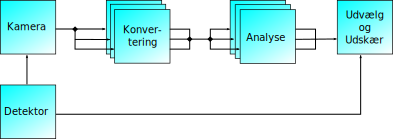
\includegraphics[scale=1]{images/pig-network3}
	\caption{Procesnetværk med flere konverteringsprocesser, og analyseprocesser}
	\label{fig:pig-network3}
\end{center}
\end{figure}
